\section{Variable compleja}
El conjunto de los números complejos se denota $\C$, y topológicamente equivale a $\R[2]$
\[ \mathbb{C} \equiv \{ (a,b) \in \mathbb{R}^2 \hspace{3px} | \hspace{3px}  a,b \in \mathbb{R} \} \]

es decir, las nociones de bolas, conjunto abierto, conjunto cerrado, compacidad y convergencia son las mismas para ambos. La diferencia recae en que a $\C$ se le dota de un producto diferente
\begin{itemize}
    \item[$\to$] $(a,b)+(c,d)=(a+c,b+d)$
    \item[$\to$] $(a,b)\cdot(c,d) = \begin{pmatrix}a&-b\\b&a\end{pmatrix}\begin{pmatrix}c\\d\end{pmatrix} = (ac-bd,ad+bc)$
\end{itemize}

% No se si poner esta info
% $[\mathbb{C},+,\cdot]$ es un cuerpo abeliano

La aplicación, $a \in \mathbb{R} \mapsto (a,0) \in \mathbb{C}$ es inyectiva y además conserva la suma y producto. Luego, $\R$ se identifica al eje $x$ en $\C$, conservando suma y producto.\\

El complejo $(0,1)$ se denomina la unidad imaginaria y se denota con la letra $i$. Cumple $i^2 = -1$, además permite escribir los complejos como

\[z = (x,y) = x + iy\]
Con $\mathrm{Re}(z) = x$ la parte real, e $\mathrm{Im}(z)=y$ la parte imaginaria.\\

\noindent 
Se definen
\begin{itemize}
    \item El conjugado de $z = x + iy$ como: $\Bar{z} = x-iy$ 
    \item Módulo de $z$ como: $\abs{z} = \sqrt{z\Bar{z}} = \sqrt{x^2 + y^2}$
\end{itemize}

\subsection{Topología}

Es exactamente la misma que en $\R[2]$, donde

\begin{itemize}
    \item[-] Sea $n \in \mathbb{N}$, $z_n = (x_n, y_n) = n_n + iy_n \longrightarrow z = (x, y) 
    \iff \begin{cases} 
    &x_n \longrightarrow x\\ 
    &y_n \longrightarrow y
    \end{cases}$ 

    \item[-] Si $f: \Omega \subseteq \C \to \C$ es una función compleja, de $z = (x, y) \in \C$ tal que $z = (x, y) \mapsto f(z)$ de variable compleja $z = x + iy$, se puede mirar como una función de 2 variables $(x,y)$ a valores en $\R[2]$, esto es
    \[ f(z) = f(x,y) = \lados{(}{u(x,y), \hspace{2px} v(x,y)} = u(x,y) + iv(x, y) \]
    Con $u,v: \Omega \subseteq \R[2] \to \R$ y $\mathrm{Re}(f) = u$ y $\mathrm{Im}(f) = v$.\\

    $f$ es continua en $z_0 = (x_0, y_0) \in \Omega \iff u,v$ son continuas en $(x_o, y_o)$
 
\end{itemize}

% Será esto necesario?
\subsection{División}
Como $\lados{[}{\C, +, \cdot}$ es un cuerpo, $\forall z \in \C, \hspace{2px} \exists z^{-1}$ inverso multiplicativo tal que $z\cdot z^{-1} = z^{-1}\cdot z = 1$. Con esto se define la división en $\C$ como
\[ \forall z_1,z_2 \hspace{2px}; \hspace{2px} z_2 \ne 0 \quad \frac{z_1}{z_2} = z_1\cdot z_2^{-1}\]

\subsection{Representación en polares}

\begin{minipage}{0.5\textwidth}%
    \begin{figure}[H]
        \centering
        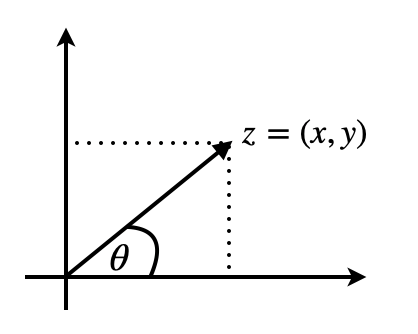
\includegraphics[width=0.58\textwidth]{CAA/Variable Compleja/en_polares.png}
        \caption{Representación gráfica}
    \end{figure}
\end{minipage}%
\begin{minipage}{0.5\textwidth}%
    \begin{equation}
        \begin{split}
            &y = \abs{z}\sin{(\theta)}\quad ;\quad x = \abs{z}\cos{(\theta)}\\
            &\theta = \mathrm{arctg}\lados{(}{\frac{y}{x}}\quad \quad \text{si } x \ne 0\\
            &z = \abs{z}(\cos{(\theta)} +i\sin{(\theta)}) = \abs{z}e^{i\theta}\\
            &\mathrm{arg}(z) = \theta
        \end{split}
        \nonumber
    \end{equation}
\end{minipage}%

\subsection{Derivadas en $\C$}
Sea $f = u +iv:\Omega \in \C \to \C$ una función compleja, y sea $z_0 \in \C$. Diremos que $f$ es derivable en $z_0 = (x_0, y_0)$ en el sentido complejo, si solo si,

\[ f'(z_0) = \lim_{z \to z_0} \frac{f(z) - f(z_0)}{z-z_0} \]

\subsection{Teorema: Condiciones Cauchy-Riemann}
Sea $f = u +iv:\Omega \in \C \to \C$ una función compleja es derivable en el sentido complejo en $z_0 \in \Omega $, si solo si, $ f = \begin{pmatrix}u\\v \end{pmatrix}$ es diferenciable en $(x_0, y_0)$ y cumplen las condiciones de C-R:

\begin{equation}
\begin{split}
    \parfrac{u}{x}(x_0,y_0) &= \parfrac{v}{y}(x_0, y_0)\\
    \parfrac{u}{y}(x_0, y_0) &= -\parfrac{v}{x}(x_0, y_0)
\end{split}
\nonumber
\end{equation}
\hfill\\
\[\implies f'(z_0) = \parfrac{u}{x}(x_0,y_0) + i \parfrac{v}{x}(x_0,y_0) = \parfrac{v}{y}(x_0,y_0) - i \parfrac{u}{y}(x_0,y_0)\]

\begin{itemize}
    \item Si $u$ y $v$ cumplen las condiciones de Cauchy-Riemann, se dice que son conjugadas. Además, si son de clase $\mathcal{C}^2$, se verifica que
    \[\nabla^2 u = \nabla^2 v = 0\]
\end{itemize}

\subsubsection{En Coordenadas Polares}

Para una función compleja expresada en coordenadas polares, $f(z)=u(r\cos{\theta},r\sin{\theta})+iv(r\cos{\theta},r\sin{\theta})=\mu(r,\theta)+i\nu(r,\theta)$, donde $z = re^{i\theta}$, las condiciones Cauchy-Riemann son

\begin{equation}
\begin{split}
    \frac{1}{r}\parfrac{\nu}{\theta}
    &=\parfrac{\mu}{r}\\
    \frac{1}{r}\parfrac{\mu}{\theta}
    &=-\parfrac{\nu}{r}\\
\end{split}
\nonumber
\end{equation}

y la derivada queda expresada como

\[f'(z)=\cos{\theta}\parfrac{\mu}{r}-
\frac{\sin{\theta}}{r}\parfrac{\mu}{\theta}+
i\lados{(}{\cos{\theta}\parfrac{\nu}{r}-
\frac{\sin{\theta}}{r}\parfrac{\nu}{\theta}}\]

\subsubsection{Función holomorfa}
Si $f:\Omega \subseteq \C \to \C$ es derivable en todo $z_0 \in \C$, se dice que $f$ es holomorfa en $\Omega$ y se denota como $f \in H(\Omega)$.\\


Si $\Omega$ es un abierto conexo y $f$ verifica que $f'(\Omega)=0$, entonces $f$ es constante en $\Omega$.

\subsubsection{Propiedades de la derivada}
Sean $f,g:\Omega \to \C$ dos funciones derivables en $z_0$, se cumple que
\begin{enumerate}[label=\roman*.]
    \item $(\alpha f + g)'(z_0) = \alpha f'(z_0) + g'(z_0) \quad; \alpha \in \C$
    \item $(fg)'(z_0) = f'(z_0)g(z_0) + f(z_0)g'(z_0)$
    \item $g(z_0) \ne 0 \Rightarrow \lados{(}{\frac{f}{g}}'(z_0) = \frac{f'(z_0)g(z_0) - f(z_0)g'(z_0)}{g^2(z_0)}$
    \item $(g \circ f)'(z_0) = g'(f(z_0))\cdot f'(z_0)$
\end{enumerate}

\subsection{Serie de Potencias}

% Quizá debería agregar una sección de series en R | También creo que sería bueno

Sean $\{c_k\}_{k\in\N}\subseteq\C$ una sucesión y $a\in\C$ una constante, para $z\in\C$, se define una suma parcial como

\[S_N(z)=\sum^N_{k=0}c_k(z-a)^k\]

El radio de convergencia de $S_N(z)$ está dado por

\[R=\lados{(}{\limsup_{k\to\infty}|C_k|^{1/k}}^{-1}\]

\begin{itemize}
    \item $S_N(z)$ converge si $|z-a|<R$, y diverge si $|z-a|>R$.
    \item Si $|z-a|=R$, $S_N(z)$ puede o no converger.
    \item La serie
    \[S(z) = \sum_{k\in\N}c_k(z-a)^k\]
    es holomorfa en $\{z\in\C\,|\,|z-a|<R\}$ con derivada
    \[S'(z) = \sum_{k\in\N}kc_k(z-a)^{k-1}\]
\end{itemize}

\subsection{Función Exponencial}

La función exponencial, $\exp:\C\to\C$, se define como

\[e^z=\sum_{k\in\N}\frac{z^k}{k!}\]

La exponencial compleja verifica que

\begin{itemize}
    \item $\forall x,y\in\R:\,e^{x+iy}=e^x(\cos{y}+i\sin{y})$
    \item $\forall z\in\C\,\forall k\in\Z:\,e^z=e^{z+2\pi ki}$
\end{itemize}

\subsection{Funciones Hiperbólicas}

\subsubsection{Coseno Hiperbólico}

Sean $x,y\in\R$, $z = x+iy\in\C$, se define la función $\cosh: \C \to \C$ como

\begin{equation}
\begin{split}
    \cosh{z} &= \frac{e^z+e^{-z}}{2}\\
    &= \sum^{\infty}_{k=0}\frac{z^{2k}}{(2k)!}\\
    &= \cosh{x}\cos{y}+i\sinh{x}\sin{y}\\
\end{split}
\nonumber
\end{equation}

\begin{itemize}
    \item $\forall z\in\C\,\forall k\in\Z:\,\cosh{(z)}=\cosh{(z+2\pi ki)}$
    \item $\cosh{z} = 0\Leftrightarrow z = \lados{(}{\frac{\pi}{2}+k\pi}i \quad k\in\Z$
\end{itemize}

\subsubsection{Seno Hiperbólico}

Sean $x,y\in\R$, $z = x+iy\in\C$, se define la función $\sinh: \C \to \C$ como

\begin{equation}
\begin{split}
    \sinh{z} &= \frac{e^z-e^{-z}}{2}\\
    &= \sum^{\infty}_{k=0}\frac{z^{2k+1}}{(2k+1)!}\\
    &= \sinh{x}\cos{y}+i\cosh{x}\sin{y}\\
\end{split}
\nonumber
\end{equation}

\begin{itemize}
    \item $\forall z\in\C\,\forall k\in\Z:\,\sinh{(z)}=\sinh{(z+2\pi ki)}$
    \item $\sinh{z} = 0\Leftrightarrow z = k\pi i \quad k\in\Z$
    \item $\cosh^2z-\sinh^2z = 1$
\end{itemize}

\subsection{Funciones Trigonométricas}

\subsubsection{Coseno}

Sean $x,y\in\R$, $z = x+iy\in\C$, se define la función $\cos: \C \to \C$ como

\begin{equation}
\begin{split}
    \cosh{z} &= \sum^{\infty}_{k=0}\frac{(-1)^{k}z^{2k}}{(2k)!}\\
    &= \frac{e^{iz}+e^{-iz}}{2}\\
    &= \cosh{iz}\\
    &= \cosh{y}\cos{x}-i\sinh{y}\sin{x}\\
\end{split}
\nonumber
\end{equation}

\subsubsection{Seno}

Sean $x,y\in\R$, $z = x+iy\in\C$, se define la función $\sin: \C \to \C$ como

\begin{equation}
\begin{split}
    \cosh{z} &= \sum^{\infty}_{k=0}\frac{(-1)^{k}z^{2k+1}}{(2k+1)!}\\
    &= \frac{e^{iz}-e^{-iz}}{2i}\\
    &= \frac{\sinh{iz}}{i}\\
    &= \cosh{y}\sin{x}-i\sinh{y}\cos{x}\\
\end{split}
\nonumber
\end{equation}

\subsection{Logaritmo}

Se define la función $\log: \C\setminus\{0\}\to\C$ como

\[\log{z} = \ln{\|z\|}+i\mathrm{arg}(z)\]

\begin{itemize}
    \item $e^{\log{z}}= z$
    \item $\log{z_1z_2}=\log{z_1}+\log{z_2}\quad\mathrm{mod}\,2\pi i$
    \item $\log$ es discontinua en $\R$
    \item $\log$ es holomorfa en $\C\setminus\R$
\end{itemize}

\subsection{Integrales}

Sean, $A\subseteq\C$ un abierto; $\Gamma\subseteq A$ una curva regular por pedazos, con parametrización $\gamma: [a, b]\to\C$; y $f:A\to\C$ una función continua, se define la integral compleja de $f$ sobre $\Gamma$ por

\[\int_\Gamma f(z)\,dz = \int^b_a f(\gamma(t))\gamma'(t)\,dt\]\\

Para $f(z) = u(x,y) + iv(x,y)$ se verifica que

\[\int_\Gamma f(z)\,dz = \int_\Gamma (u\hat{x}-v\hat{y})\cdot d\Vec{r}+i\int_\Gamma (v\hat{x}+u\hat{y})\cdot d\Vec{r}\]

\newpage